\section{InterProScan as Supporting Evidence for Predicted Genes}

Pfam hits from InterProScan analysis are presented in table
~\ref{ips-pfam:table}, from which we can identify one major trend. In
general, between 65 and 75 percent of proteins predicted by both
Braker2 and GeneMark contain a match to a Pfam entry. This is
promising performance for the gene finders as the RefSeq annotations
demonstrate similar proportions of Pfam hits to predicted
proteins. The total counts may be decieving however, as predictions
from Braker2 may result in more than one protein product. In the case
of GeneMark, only one protein is produced per gene model. From visual
inspection of Pfam hits mapped back to the references, it would appear
that in general, when gene finders agree that a gene is present,
InterProScan reports the same Pfam match in all three predictions. An
example of agreement between Braker2, GeneMark, RefSeq and
InterProScan is shown in figure \ref{fig:basic-agree}. 

\begin{table}[!]
  \centering
  \begin{tabular}{|c|c|c|c|c|c|c|}
    \hline
    Assembly & \makecell{Braker \\ Proteins} & \makecell{Braker Pfam \\ Hits} & \makecell{GeneMark \\ Proteins} & \makecell{GeneMark Pfam \\Hits} & \makecell{RefSeq \\ Proteins} & \makecell{RefSeq Pfam \\ Hits}  \\ \hline
    DC1 & 14479 & 10676 & 11354 & 8416  & N/A & N/A \\ \hline
    Tsth20 & 15546 & 11389 & 12373 & 9168 & N/A & N/A \\ \hline
    \textit{T. reesei} & 11704 & 8471 & 9196 & 6990 & 9111 & 6964 \\ \hline
    \textit{T. harzianum} & 15408 & 11370 & 12164 & 9061 & 14065 & 9293 \\ \hline
    \textit{T. virens} & 15062 & 11249 & 11866 & 8871 & 12383 & 9062 \\ \hline
  \end{tabular}
  \caption[InterProScan Pfam Evidence]{Table with counts of predicted
    genes with Pfam annotations from InterProScan}
  \label{table:regioncounts}
\end{table}


\begin{figure}
  \centering
  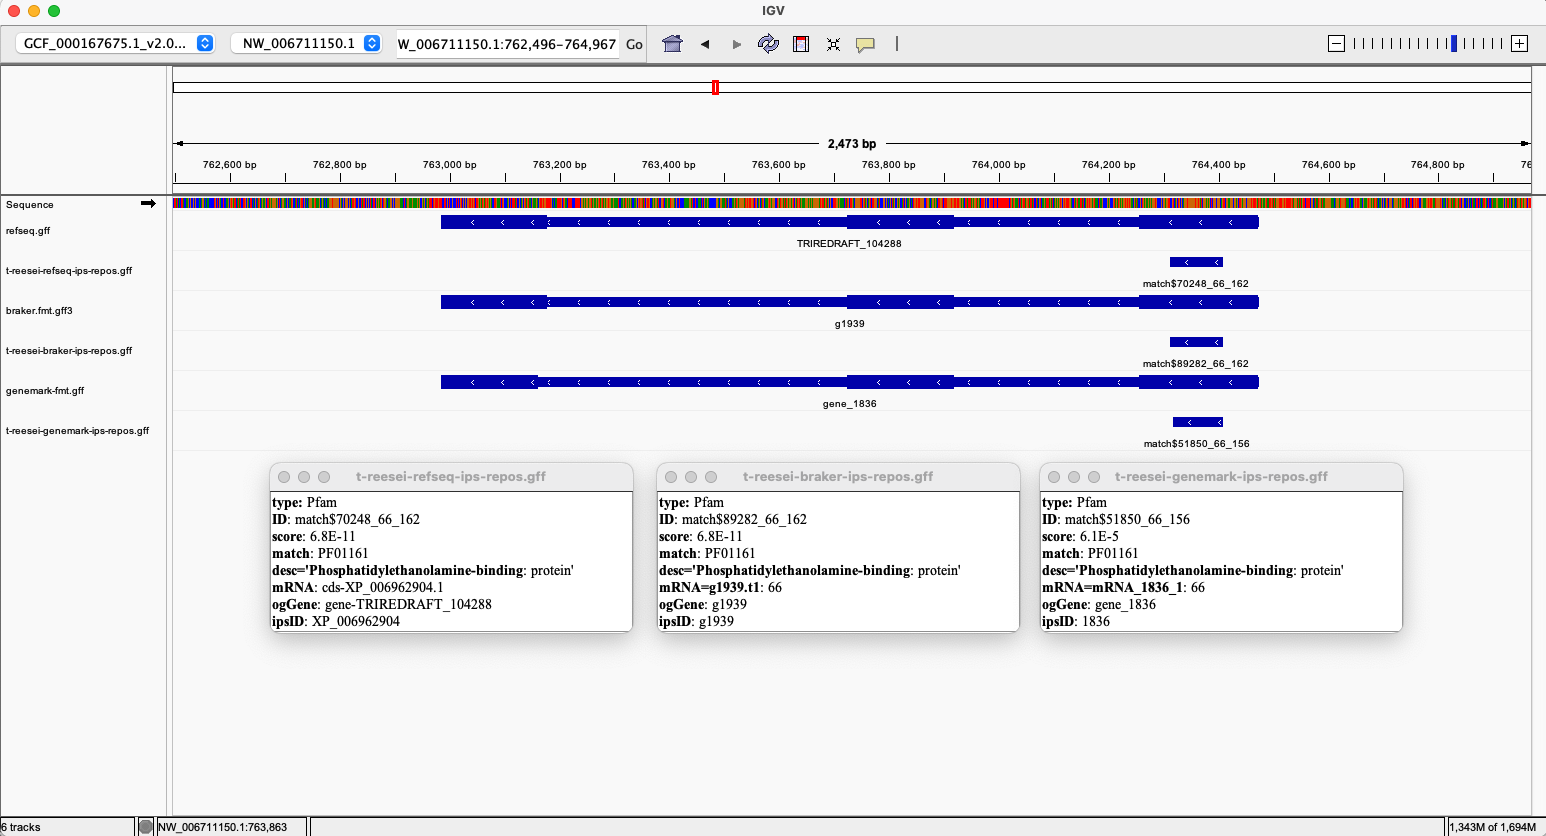
\includegraphics[width=0.8\textwidth]{figures/igv/ips-basic-agree.png}
  \caption[Agreeing Pfam matches]{An IGV capture showing complete
    agreement between gene finders for both gene model and protein
    Pfam hits}
  \label{fig:basic-agree.png}
\end{figure}

While cases of complete agreement are abundant, cases of disagreemnt
also exist and in strange forms. In many cases, while the gene finders
agree on the presence of a gene, only the RefSeq protein product
contains a match to the Pfam database. Why this may be the case is
unclear, and may warrant further investigation. There are also many
cases in which InterProScan reports the same Pfam hits, but the gene
models in the region do not agree. There are even cases such as the
region shown in figure \ref{fig:agree-bizarre2}, where Braker2 and
GeneMark agree that two genes andtheir associated proteins and Pfam
matches are separate, but RefSeq only reports one gene with multipl
Pfam hits.

\begin{figure}[!]
  \centering
  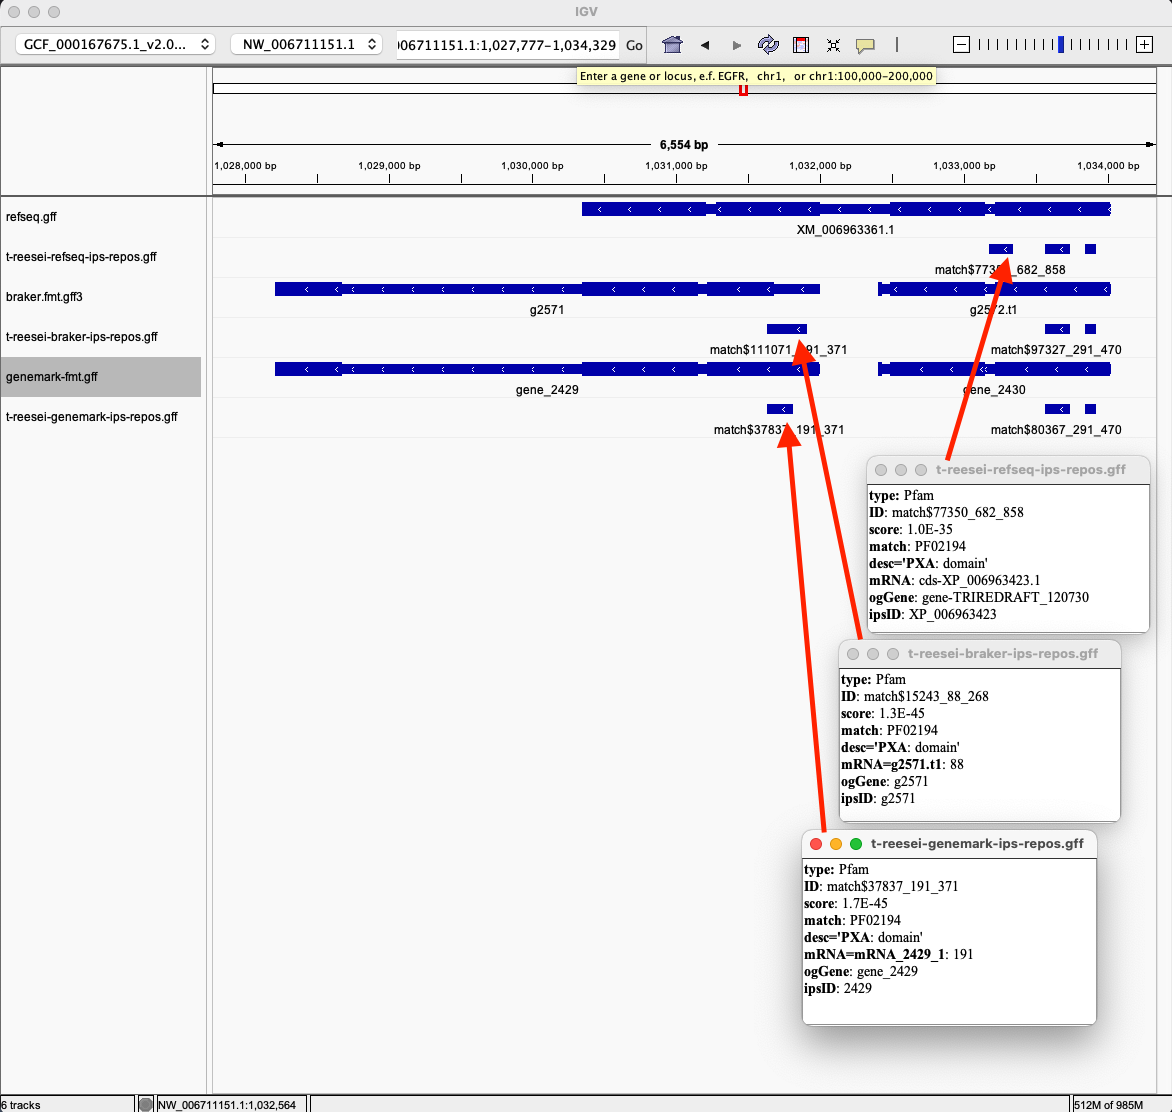
\includegraphics[width=0.8\textwidth]{figures/igv/ips-model-disagree2.png}
  \caption[Split Pfam matches]{An IGV capture showing Braker2 and
    GeneMark reporting two genes and their resulting proteins and
    Pfam hits as separate, while RefSeq reports one gene, one protein
    and three Pfam matches.}
  \label{fig:agree-bizarre2}

\end{figure}
